\chapter{Behavioural modelling of pedestrian movement using novel data sources and machine learning}
\label{chap6}
\chaptermark{Interactions of Pedestrians and Automated Vehicles: Trajectory}
\addtocontents{toc}{\protect\setcounter{tocdepth}{1}}
\thispagestyle{empty}
\pagebreak

\section*{Preamble}
This chapter features another aspect of the pedestrian crossing behaviour in automated environments of future urban space: trajectory. Utilizing data retrieved from the same virtual reality experiment described in the previous chapter, data-driven time-series models are developed to predict the trajectory of pedestrians while crossing roads confronting automated vehicles. The model uses the initial movements of pedestrians, as well as their head orientations and distance to the coming vehicle as input, and merges them with contextual information of the environment to predict the location of the next steps of pedestrians. All the input to the models are set in a way that can be captured by a hypothetical automated vehicles, making it possible to predict the movements of pedestrians based on the information that are available to a typical automated vehicle. This chapter also include an extensive review of the available open-source datasets related to real test automated vehicles on the roads, and discusses their drawbacks and advantages from a pedestrian-oriented point of view.

\vspace{1em}
\noindent
This research article is under review in \textit{Transportation Research Part C: Emerging Technologies}
\clearpage

\section*{Abstract}

\clearpage

\section{Introduction}
\label{S:TInt}

The rapid technological development in Automated Vehicles (AVs), followed by a tremendous increase in their adoption, promises a significant transformation in the dynamics on urban roads. An important transformation expected to occur is the effect of AVs on pedestrians, as the most vulnerable road users. Particularly, in the absence of a driver in the vehicles, and thus the absence of eye contact and observation and interpretation of head and body movements by the driver, the interaction between vehicle and pedestrian has to be re-investigated to account for the resulting changes. To be able to compensate for the silent agreement between the driver and pedestrian, and establish a similar type of interactions between pedestrians and vehicles in an automated environment, AVs need to find a way to anticipate pedestrian behaviour, i.e. intentions, choices and movements/trajectories, based on the pedestrian reactions captured. Failures in the prediction of pedestrian behaviour and the absence of timely actions by the AV have already resulted in catastrophic accidents in recent years, even at very slow speeds~\citep{uber,vienna}.

Studying pedestrian behaviour is an active and extensive area of research. In this study, however, we focus on behaviour of pedestrians when crossing mid-block, unsignalized roads. As rule-obeying AVs find their way on the streets in future urban spaces, it is a plausible scenario that this type of crossing increase in spatio-temporal frequency~\citep{millard2018pedestrians}. Going through the official reports of uber's test AV incidence in Arizona, it appeared that the vehicle's system could not predict the pedestrian's path correctly because she was crossing mid-block, and \textit{"the system design did not include consideration for jaywalking pedestrians."}~\citep{uber,ntsb}. Thus, a thorough investigation of mid-block crossings is timely and of vital importance. 

We can simplify the interactions of an AV and a pedestrian crossing mid-block to three parts~\cite{kalatian2020decoding}. As depicted in \cref{fig:Tinteraction}, (a) a pedestrian waits on the sidewalk for the right time to initiate a cross, (b) They then follow a certain trajectory based on the characteristics of the approaching vehicle, and geometric and environmental conditions. On the other hand, the vehicle anticipates pedestrian behaviour and reacts to it by making the required decisions to provide a safe and comfortable crossing for the pedestrian while accounting for the passengers' safety and comfort. We explored the first part of this interaction, i.e., wait time of pedestrian, in two previous studies~\cite{kalatian2019deepwait,kalatian2020decoding}. Here the focus is to understand and develop prediction models for the second part, the pedestrian trajectory. Together, the two behaviour prediction models can then be used by AVs to anticipate pedestrian movement better and proactively make maneuvering decisions~\cite{vasquez2019multi}.

\begin{figure}
    \centering
    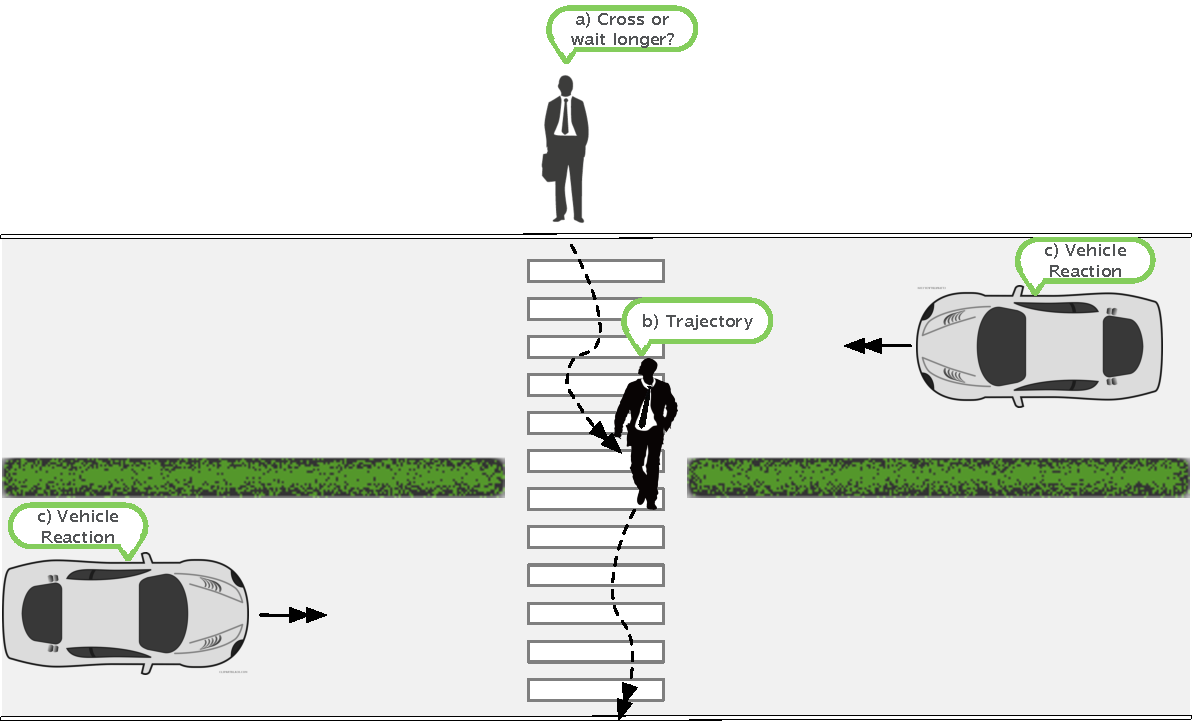
\includegraphics[scale=0.7]{chapter_6/figures/cross.pdf}
    \caption{Schematic representation of vehicles and pedestrians interactions}
    \label{fig:Tinteraction}
\end{figure}

Given an initial observation of the behaviour, as well as contextual information of the environment in which the crossing takes place, we developed a prediction model to estimate the trajectory of a pedestrian. By providing an extensive review of the open-access AV datasets, we discuss existing gaps within them. Data used to train and test the models in this study are collected using the Virtual Immersive Reality Environment (VIRE)~\cite{farooqvire} framework. Virtual Reality (VR) tools have made it possible to create an immersive and controlled environment in which detailed pedestrian behaviour can be analyzed under specific sets of conditions.. 

A novel multi-input network of Long Short-Term Memory (LSTM) and fully connected dense layers is developed to model trajectories of pedestrians while they cross a road in an automated environment. In the proposed model, time-series data of the initial steps of crossing, including trajectories, head orientations, and distance to vehicles, are added to non-time-series data of contextual information of the crossing's environment to predict the next steps of pedestrian trajectories. A game theory-based post-hoc interpretability method for neural networks is applied to analyze the contributing factors to pedestrian trajectory prediction. By providing insights into the most determining factors in trajectory prediction, we propose suggestions that can help to improve currently available datasets from a pedestrian-oriented point-of-view.  

The rest of this paper is organized as follows: a review of relevant studies in trajectory prediction and an extensive review of currently available open-access AV datasets are provided in the next section. \cref{S:t3} briefly discusses data collection and pre-processing procedures. Methodology and proposed architecture are described in \cref{S:t4}. The application of our proposed framework on the data and their interpretation are discussed in \cref{S:t5}. Finally, \cref{S:t6} is dedicated to conclusions, final remarks, and future research plans of the project.

\section{Background}
\label{S:tBack}
This section provides an overview of the research studies on pedestrian crossing behaviour, emphasizing trajectory prediction studies. Traditional approaches to pedestrian trajectory modelling and recent data-driven trends are discussed in this chapter. Modern data-driven approaches require novel large-scale datasets. In order to understand pedestrian behaviour in the presence of AVs, real datasets from AV manufacturers are the most reliable resources. Thus, a review of the available datasets from a pedestrian-oriented point-of-view is provided, followed by a discussion on data alternatives for AV-pedestrian studies.      
\subsection{Pedestrian trajectory prediction}
Early models in the literature tried to model the pedestrian movement using the concepts and theories of ideal gases~\cite{henderson1974fluid} or fluids~\cite{helbing1998fluid}. However, the turning point in pedestrian movement modelling was the social force model by Helbing and Molnar in 1995~\cite{helbing1995social}. Based on the idea that behavioural changes are caused by so-called social fields, Helbing and Molnar described forces affecting pedestrian behaviour as a result of internal motivations of an individual to decide and perform actions. In 2004, Antonini~\textit{et al.} applied logit-type discrete choice models to pedestrian movement analysis using video data~\cite{antonini2004simulation}. The microscopic approach of the model allowed a detailed analysis of pedestrian movement. The choices that a pedestrian was facing at a certain time in their model were: (1) speed level and (2) discrete radial direction. Utility functions for each of these choices were defined based on the presence of obstacles, proximity to the destination and positions and speeds of other pedestrians. Later works on these models added other variables, helping the model gain strength by of observing various factors. For instance, Guo \textit{et al.}~\cite{guo2012route} added visibility parameters to the model while Asano~\textit{et al.}~\cite{asano2010microscopic} later incorporated density. The major weaknesses of such microscopic methods using logit formulation is their requirement to discretize the space and speed into arbitrary levels. Furthermore, they are very myopic as they can only predict the next-step decision based on current conditions without incorporating what is ahead, e.g., approaching vehicle or a wall a few metres ahead.

The widespread success of machine learning methods in recent years, as well as the availability of large pedestrian datasets, have resulted in a shift of pedestrian research trends to data-driven. In particular, recurrent networks, i.e., RNN and LSTM, have been the dominant machine learning methods for trajectory prediction. In most cases, the input data used for trajectory prediction is only the past trajectory of the pedestrians~\cite{xue2019location,zhang2019sr,alahi2016social,gupta2018social}. In one of the significant earlier studies in the field, Alahi~\textit{et al.}~\cite{alahi2016social} introduced Social LSTM, a method that incorporated interactions among pedestrians in sequential models, namely Long Short-Term Memory (LSTM), to forecast trajectory of pedestrians using video footage of walking individuals in crowded scenes. In their method, a \textit{Social Pooling Layer} is added to the framework. Through this layer, LSTM layers trained for individuals in a scene share their information. In spite of the success of the Social-LSTM model in forecasting pedestrian trajectory, this model does not account for the contextual information on the environment and aspects like where the pedestrian is looking. The model may be applicable in pedestrian-dominant environments, e.g., shopping mall or train station, but is difficult to apply to situations like road crossing behaviours of pedestrians in an automated environment. Furthermore, the future trajectory predicted by Social-LSTM assumes a fixed-length future trajectory.  More recently, Gupta~\textit{et al.}~\cite{gupta2018social} introduced \textit{Social-GAN}, a model that predicts socially acceptable trajectories by training adversarial against a recurrent discriminator. Similar to~\cite{alahi2016social}, this model fails to capture context information from the environment, and its applicability is limited.

Some other research studies have incorporated contextual and semantic information into the pedestrian trajectory to predict their next locations~\cite{lee2017desire,chandra2019traphic,rasouli2019pie}. The semantic information used can be road design~\cite{bi2019joint}, the shape of objects~\cite{chandra2019traphic}, and the speed of the vehicles~\cite{bhattacharyya2018long,rasouli2019pie}. Lee~\textit{et al.}, for instance, added semantic contexts, such as road structure and interactions and dynamics of the agents to their proposed RNN model and predicted pedestrian trajectory of variable lengths in a video dataset~\cite{lee2017desire}. Despite all the diversity in models, data and objective functions in the relevant research studies, only a few models have attempted to predict pedestrian trajectory in the context of AVs. In most such cases, analyzing pedestrian is limited to crowds, and not in the context of interactions with vehicular traffic. To the best of our knowledge, almost all the models in the literature have used general-purpose video footage of pedestrian movements as the input data. Because pedestrian road crossing behaviour in the presence of AVs may differ, current datasets and scenarios may not apply to the futuristic scenarios. One of the reasons behind this gap can be traced back to the lack of pedestrian data in open-access AV datasets. In the next subsection, an overview of these datasets is provided.

\subsection{Open-Access AV datasets}
Despite the significant improvements in AVs' general operations through video and sensor datasets, pedestrian-AV interaction modelling using such datasets has not been thoroughly explored. AV datasets have been widely explored for object detection~\cite{chang2019argoverse}, semantic segmentation~\cite{porzi2019seamless}, and vehicle trajectory prediction~\cite{gu2020lstm,chandra2020forecasting,lee2017desire}. However, a lack of pedestrian behavioural studies using these open-access AV datasets made us explore the gaps and missing components in these datasets. In the rest of this subsection, an overview of four available open-access automated datasets is provided from a pedestrian-oriented point-of-view. 
\subsubsection{NuScenes}
With 1,000 scenes of 20 seconds each~\cite{nuscenes2019}, nuScenes is one of the largest open-access dataset available for AV research. The vehicle containing sensors (ego vehicle) in nuScenes' data collections is equipped with 6 cameras, 1 LIDAR\footnote{Light Detection and Ranging sensor} and 5 RADAR, GPS, and IMU\footnote{Inertial Measurement Unit sensors} sensors as the entire sensor suite of an AV. With around 5.5 hours of driving in congested urban areas of Boston and Singapore, nuScenes is a suitable match for studying modern urban spaces. Twenty-three classes of objects are annotated in the dataset, including pedestrians, children, bicycles, construction zones, etc. High-quality annotations of pedestrians make it easier to extract relevant frames from the dataset and focus on the pedestrian side of the scenes. With detailed information on the ego vehicle position, the dataset enables finding the vehicle-to-pedestrian distance at each time frame. Although the dataset is inclusive in different weather conditions, vegetation, and road markings, such information is not provided in the dataset and needs to be extracted by processing frames and videos. Including the underlying maps of the ego vehicle is another advantage that the nuScenes dataset provides, enabling extracting some context from the map. \cref{fig:nusc} shows a sample image from different cameras of a nuScenes ego vehicle.
\begin{figure}
    \centering
    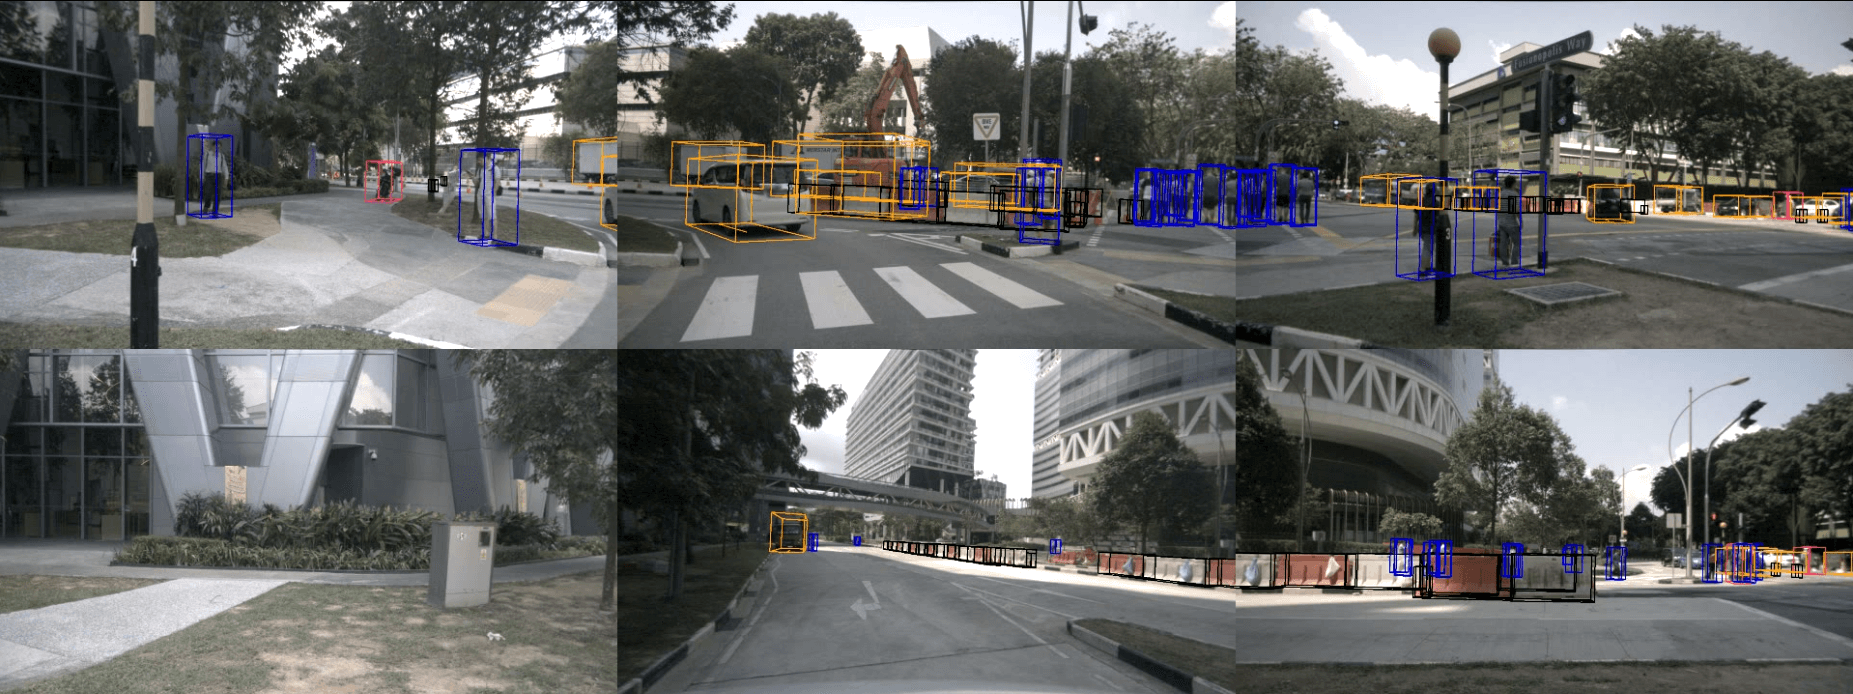
\includegraphics[scale=0.2]{chapter_6/figures/nusc.png}
    \caption{Object annotation example in nuScenes dataset (photo from \href{https://www.nuscenes.org/}{nuScenes})}
    \label{fig:nusc}
\end{figure}

\subsubsection{Lyft Level 5 open data}
Built upon the nuScenes database schema, Lyft level 5 dataset provides 2.5 hours of automated driving in Palo Alto, California~\cite{lyft2019}. Similar to nuScenes, underlying maps, annotations and different weather conditions are included in the dataset. Although it is relatively new, using the same database format as nuScenes gives Lyft level 5 dataset a robust and well-documented structure.  
\cref{fig:lyft} depicts a schematic image of a Lyft automated vehicle and its sensors.
\begin{figure}
    \centering
    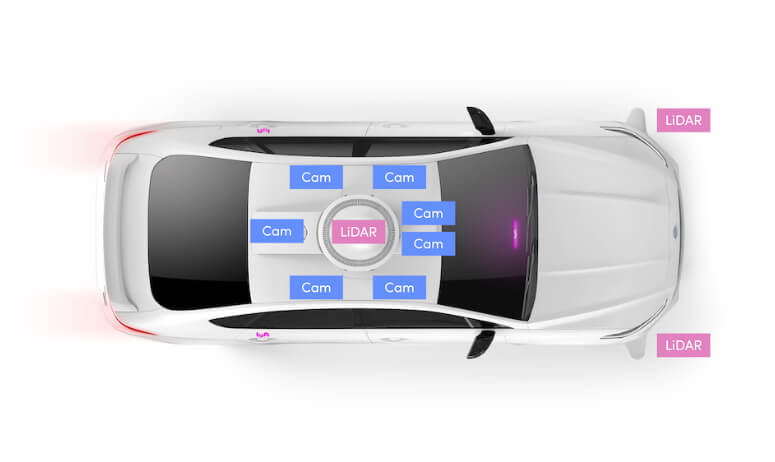
\includegraphics[scale=0.5]{chapter_6/figures/lyft.jpg}
    \caption{A schematic representation of a Lyft ego vehicle with all its sensors locations (photo from \href{https://self-driving.lyft.com/level5}{Lyft})}
    \label{fig:lyft}
\end{figure}  
\subsubsection{Waymo}
As of November 2020, Google's Waymo dataset is the largest and most annotated AV data available~\cite{sun2020scalability}. With  1150 scenes of over 6 hours of driving, the covered 76 $km^2$ area in the Waymo dataset is the largest among all the available datasets. Using three coordinate systems and providing means to transform data between frames, it is easy to follow and extract the trajectories of objects by having the positions of objects both in global coordinates and vehicle frame (relative to the ego vehicle position). Extensive hours of data collection include driving in various scenarios, including night time and daylight, construction areas, downtown and suburban areas, and diverse weather conditions. The recordings have been captured in Phoenix, Mountain View and San Francisco, enabling research opportunities in domain adaptations. The database format used for Waymo is new and different from those of other datasets, making the application of the models designed based on other datasets require further data cleaning procedures. However, having an active GitHub community with strong documentation helps smooth this transition. Unlike other popular AV datasets, the Waymo dataset currently does not include an underlying map of the events, making utilization of semantic information of the map in the algorithms impossible.   
\cref{fig:waymo} shows an annotated LIDAR data sample from Waymo dataset.
\begin{figure}
    \centering
    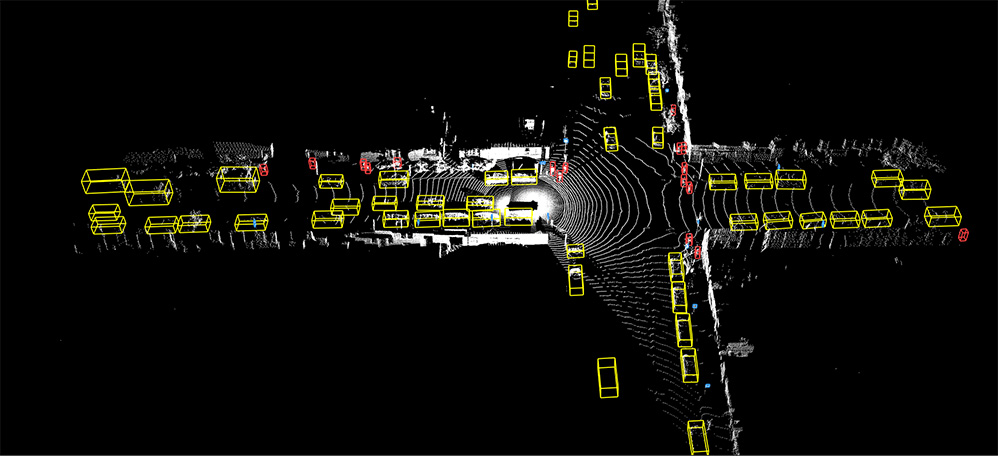
\includegraphics[scale=0.4]{chapter_6/figures/waymo.jpg}
    \caption{An annotated LIDAR data sample (photo from \href{https://waymo.com/open/data/}{Waymo})}
    \label{fig:waymo}
\end{figure}    

To study unsignalized crossing behaviour of pedestrians, we investigated NuScenes, Waymo and Lyft level 5 datasets to extract the relevant frames to the objective of this study.

\subsubsection{Pedestrian crossing in AV datasets}
We extracted pedestrian instances based on the LIDAR data of Lyft, nuScenes and Waymo dataset, and the annotations provided. We defined seven criteria and applied them to the datasets to narrow down to events involving mid-block crossings of pedestrians. The defined criteria are:
\begin{enumerate}
    \item Pedestrian is detected in front of the car: as LIDAR data enables detection of pedestrians even if they are on the rear side, a proportion of pedestrians detected are not interacting with the ego vehicle when during the scene. This filter makes sure that the ego vehicle is or will interact with the pedestrian during the scene
    \item Pedestrian is seen on both left and right sides of the ego vehicle: to limit the event to pedestrian crossings, it is expected that during the scene, the pedestrian is detected on both sides of the ego vehicle
    \item Pedestrian is moving in front of the ego vehicle: remove instances of pedestrians waiting, waling on the sidewalk, sitting, etc.
    \item Trajectory of detected pedestrians form an angle of 45 to 135 degrees with the trajectory of the ego vehicle
    \item Ego vehicle's change of direction forms an angle of less than 60 degrees. This filter is added to avoid turning vehicles to be included as they might pass all the previous criteria with no crossing of pedestrian taking place
    \item The distance between a pedestrian and the ego vehicle is less than 50 meters
    \item Pedestrian and ego vehicle have intersecting trajectories meaning that they path a similar point during the scene
\end{enumerate}
It should be noted that due to the short length of scenes, the last criteria should be loosened as ego vehicle might not necessarily pass the points that pedestrian is observed. The scenes related to remained data are then manually observed to verify if a pedestrian is crossing mid-block in front of the ego vehicle.

We start with the Lyft dataset, as the smallest dataset of all. In total, 350 scenes were available within the original dataset. Not considering the distance, and applying the first five filters, 137 possible instances of jaywalking pedestrians are found. However, when the instances are limited to a 50-meter maximum distance between pedestrian and ego vehicle, only 20 instances remain. After carefully watching the 20 remained instances, it appeared that no jaywalking events occurred within the dataset. The relatively short 2.5 hours length of the Lyft dataset can be mentioned as the reason behind the failure to find any instances. 

Moving forward to nuScenes dataset with the same format as Lyft level 5, 5.5 hours of driving is available in nuScenes dataset, leading to a compressed size of 350 GB. After tracking and detecting pedestrians among different frames of scenes using annotation IDs, 8,143 unique pedestrians were found and tracked in the dataset. After applying all the criteria defined, 200 of the instances remain in the dataset. However, by viewing the videos of the remaining instances, it appears that further filters are required in order to extract jaywalking instances more accurately. For example, in some instances the ego vehicle is interacting with a pedestrian in a parking lot or a private driveway. Although such instances meet the criteria define in our filters, they cannot be categorized as mid-block crossing events. Having more information about the environment that the ego vehicle is driving can help distinguish such instances automatically without the need for manual subjective observations or complex video processing. 

Finally, the Waymo dataset was investigated to extract crossing pedestrian events. In the first step, an impressive number of 23,056 unique pedestrians were tracked between the frames. However, only 1,182 of the total pedestrians passed filter 1 and were detected in front of the car. By applying filter 2, 280 of the remaining pedestrians passed the criteria of being observed on both sides of the ego vehicle. One hundred of the remaining pedestrians were removed from the data by adding the walking filter, leading to 211 instances of potential mid-block crossings. By applying the angle criteria, 117 pedestrians were left in the dataset. However, when observing the video data of the remaining instances, it appeared that a major part of the crosses was related to ego vehicle turning events, which made the walking pedestrians on the sidewalks pass all the previous filters. By introducing filter 5 and focusing on vehicles following a relatively straight trajectory, only 55 instances were left in the dataset.

By investigating some of the most well-established open-access AV datasets it appears that in order to extract events of a specific behaviour of pedestrians, larger and more extensive datasets are required. A solution to overcome this challenge would be to combine data from different resources to create a hybrid dataset focused on pedestrians. However, difference in data formats, sensors, environments and coordinate systems used make it a challenging and difficult task to combine these datasets. Another solution would be to collect data with a particular focus on pedestrians. However, most popular video datasets used for pedestrian behaviour analysis are dedicated to pedestrian interactions with each other and their dynamics in crowds~\citep{robicquet2016learning,zhang2019widerperson}. In recent years, some researchers have tried to address this issue and collect and provide pedestrian-oriented AV datasets~\cite{dipietro1970pedestrian,kotseruba2016joint}. However, these datasets are still not well-established in the literature. To understand the most essential context information required for pedestrian trajectory studies, we develop a controlled virtual reality experiment. The controlled nature of our data allows us to record pedestrian behaviour under several customized conditions and test the effects of various contextual information on the model accuracy.     

\section{Virtual Reality Data}
\label{S:T3}
For the purpose of this study, Virtual Immersive Reality Environment (VIRE) is used to simulate different scenarios and conduct experiments on different pedestrians safety and walking behaviour. Introduced in Farooq~\textit{et al.}~\citep{farooqvire}, VIRE uses Head Mounted Display and virtual reality to enable interactive, immersive and complex simulated scenarios. Hypothetical traffic simulations can be projected directly to eyes of users. In this study, we specifically focus on pedestrian crossing behaviour at unsignalized intersections, as a plausible scenario in the autonomous future. Participants are asked to cross the street in different scenarios.
Detailed experiments were conducted over a 3 month period in summer 2018, in four different places to cover a heterogeneous population. A total of 160 individuals from different age groups participated in the experiment. The experiments were performed at Ryerson University, City of Markham Public Library, Toronto City Hall, and North York Civic center. Participants were exposed to multiple scenarios, with changing parameters in each round. In Figure \ref{fig:exp}, an experiment and its components are shown.
\begin{figure}[!h]
\centering
\sbox{\measurebox}{%
  \begin{minipage}[b]{.4\textwidth}
  \subfloat
  {\label{fig:figA}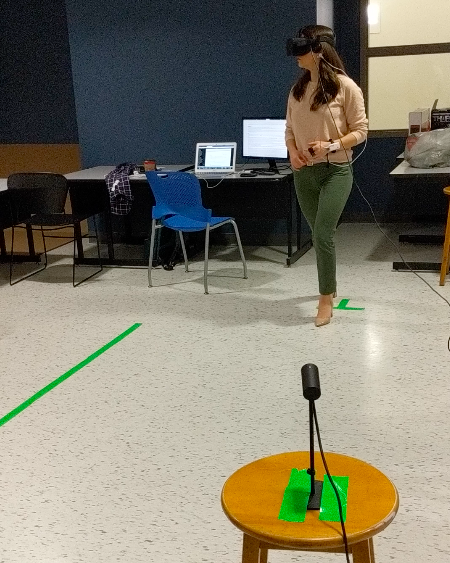
\includegraphics[width=0.91\textwidth,height=8cm]{chapter_6/figures/img1.png}}
    (a)
  \end{minipage}}
\usebox{\measurebox}\qquad
    \begin{minipage}[b][\ht\measurebox][s]{.4\textwidth}
    \centering
    \subfloat
    {\label{fig:figB}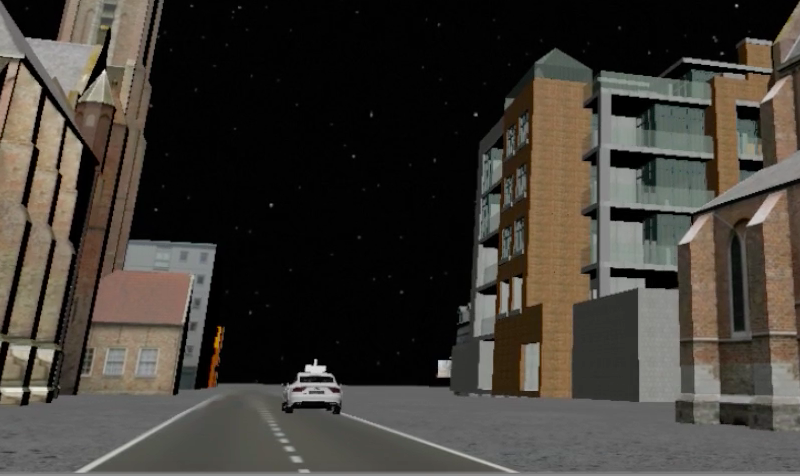
\includegraphics[width=0.91\textwidth,height=3.5cm]{chapter_6/figures/img3.png}}
    (b)
    \vfill
    \subfloat
    {\label{fig:figC}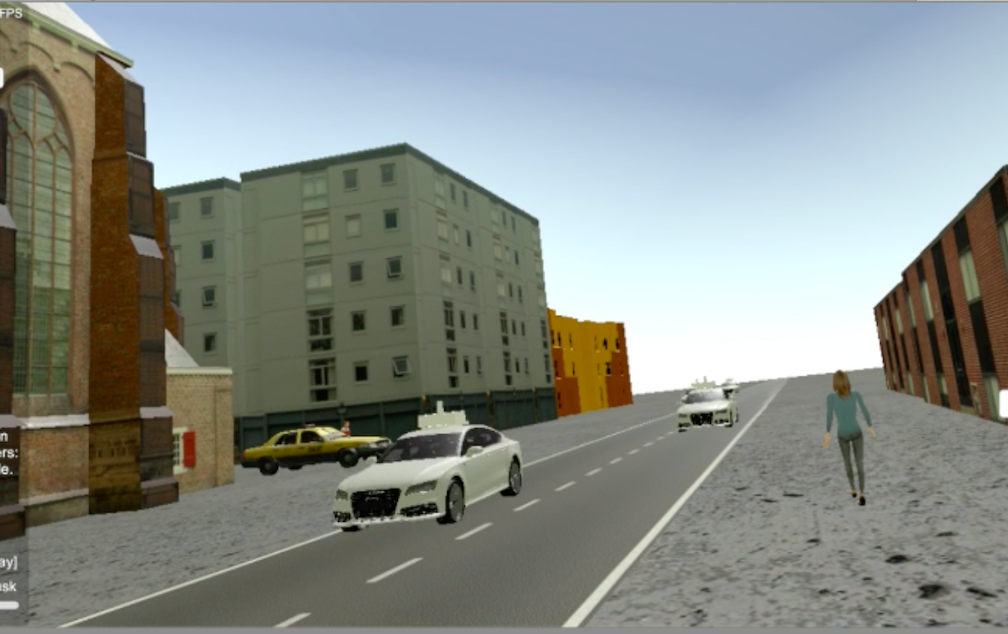
\includegraphics[width=0.91\textwidth,height=3.5cm]{chapter_6/figures/pic1.png}}
    (c)
    \end{minipage}
\caption{VR experiment. (a) A participant doing the experiment (b) A sample night view of the environment (c) A sample day view of the environment}
\label{fig:exp}
\end{figure}
While doing the experiment, pedestrians coordinates and head orientations, as well as simulated vehicles' positions are recorded every 100 milliseconds. Environmental context variables used as auxiliary input to the core LSTM network include type of road (one-way, two-way or two-way with median), speed limit (30, 40 or 50 km/hr), lane width (2.5, 2.75 or 3 m), weather conditions (snow day or clean), time of the day (day or night), and arrival rate of cars (530, 750, 1100 veh/hr). These variables are defined in a way that a self-driving car can capture and use them as input to its trajectory prediction algorithm. More information on other features used for the purpose of scenario generation and design of experiments can be found in ~\citep{kalatian2019deepsurvival}.  

\section{Methodology Description}
\label{S:t4}
Pedestrian movement patterns are highly correlated both temporally and spatially \cite{song2016deeptransport}. Recurrent Neural Networks (RNNs) are a popular choice to deal with the problem by treating mobility patterns of a pedestrian as a sequence prediction problem. However, it has been shown that RNNs are not capable of remembering long-term temporal and spatial dependencies as a result of the problem of vanishing gradient~\cite{hochreiter1997long}. Introduced in \cite{hochreiter1997long}, Long Short-Term Memory (LSTM) is a modification to traditional RNN architecture that enables learning sequence labels for longer time intervals by implementing four interactive gates. In \cref{fig:LSTM}, a schematic representation of a typical LSTM network is depicted. To compute a sequence of output units \(Y=(y_1,y_2,...,y_T)\), from a sequence of inputs \(X=(X_1,X_2,...X_T)\), the following equations should be followed iteratively over time \textit{t}:

\begin{itemize}
    \item forget gate: 
    \begin{equation}
        f_t=\sigma(W_fx_t+U_fh_{t-1}+b_f))
    \end{equation}
    \item input gate:
    \begin{equation}
    i_t=\sigma(W_ix_t+U_ih_{t-1}+b_i)
    \end{equation}
    \item Cell state:
    \begin{equation}
    c_t=f_t\odot c_{t-1}+i_t\odot \sigma(W_cx_t+U_ch_{t-1}+b_c) 
    \end{equation}
    \item output gate:
    \begin{equation}
    o_t=\sigma(W_ox_t+U_oh_{t-1}+b_o)
    \end{equation}
    \item hidden state:
    \begin{equation}
    h_t=o_t\odot \sigma(c_t)
    \end{equation}
    \item output layer:
    \begin{equation}
    y_t=\sigma(W_{y}h_t+b_y
    \end{equation}
\end{itemize}
in which: \(f_t,i_t,o_t\) are the activation vectors of forget gate, input gate and output gate respectively. \(h_t\) is the hidden state vector, which plays the role of an output vector of LSTM unit, \(c_t\) is the cell state vector, \(W,U\) and \(b\) are the weights and biases to be learned in the training phase, and \(\odot\) represents the element-wise product. \(\sigma\) represents the activation functions on respective layers. 
\begin{figure}
    \centering
    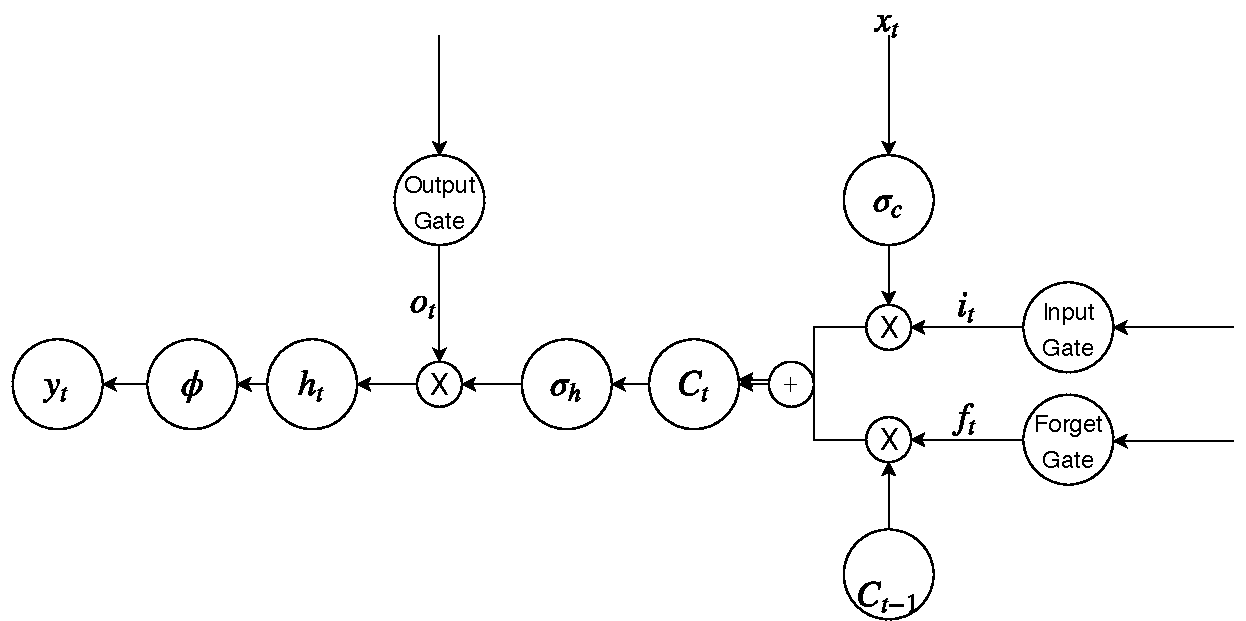
\includegraphics[scale=0.6]{chapter_6/figures/lstm.pdf}
    \caption{Schematic framework of an LSTM block}
    \label{fig:LSTM}
\end{figure}

In this study, we propose, \textit{Aux-LSTM}, a novel framework consisting of multi-input LSTM layers and fully connected dense layers, to predict the next coordinates of pedestrians as output. Initial steps of time-series data, i.e., coordinates, head orientations, and distance to vehicle, are used as input to the LSTM layers. The output of the LSTM layers will then merge with extra information from environmental variables, and the mergers enter a series of fully connected dense layers to predict the trajectory of the pedestrians in the rest of their crossing. Input time-series data are defined in two ways: time-based and distance-based. In the time-based approach, the coordinates of the pedestrian in the next $t_2$ seconds are predicted based on their last $t_1$ seconds of behaviours. At each point during the cross, pedestrian coordinates, head orientations, and their distance to the approaching vehicle during the last $t_1$ seconds are used as time-series input to predict the coordinates of the pedestrian in the next $t_2$ seconds. In the distance-based type of models, however, the proportion of data that is used as input, $p$, is defined as the proportion of lane width that the pedestrian has passed when the algorithm tries to predict the coordinates of the pedestrian in the rest of the cross. For instance, if $p$ is set to 0.3, the framework tries to predict the trajectory of the pedestrians based on their trajectory in the first 30\% of the lane width. Different values of $t_1$, $t_2$ and $p$ are tested in order to provide insights into the required method of data preparation.

As a regularization mechanism to the framework, the model is supervised through two identical loss functions. Both loss functions are defined as the euclidean distance between predicted and actual coordinates. By using the loss function after the LSTM layers, a.k.a. secondary loss, we allow smoother training for the framework. Batch Normalization and Dropout layers are also used in order to reduce overfitting in the model. \cref{fig:Tframe} depicts the general framework of Aux-LSTM.
\begin{figure}
    \centering
    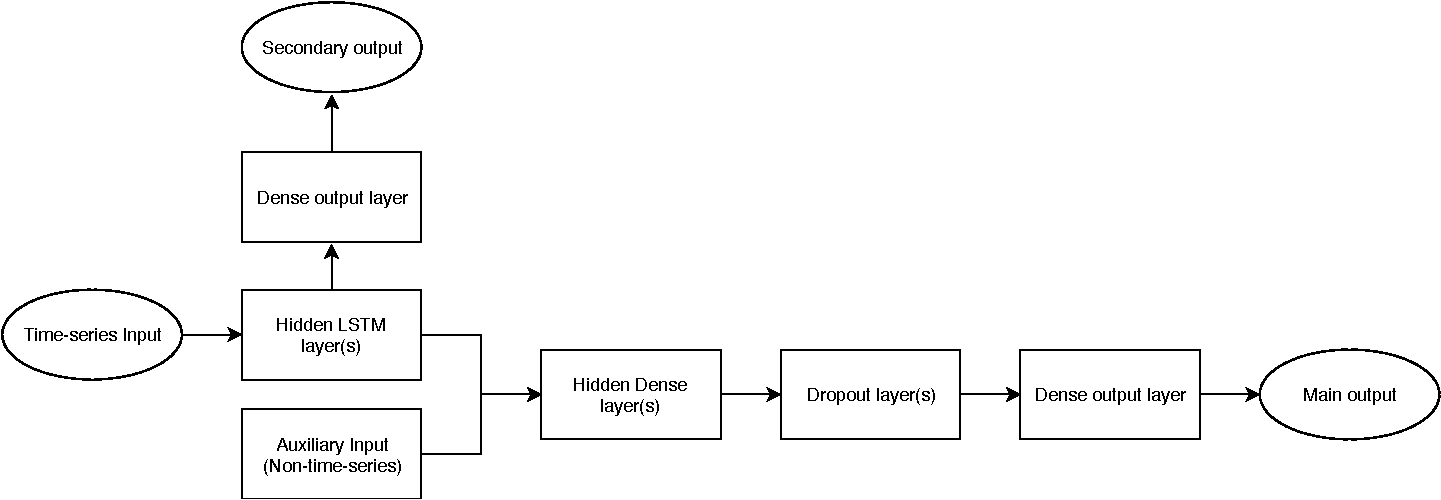
\includegraphics[scale=0.57]{chapter_6/figures/frame.pdf}
    \caption{Schematic framework of Aux-LSTM}
    \label{fig:Tframe}
\end{figure}

\section{Results and Analysis}
\label{S:T5}
\subsection{Implementation Notes}
All data pre-processing and model development are coded in Python programming language, using Keras library and its implementation of TensorFlow with GPU support. After data preparation, an exhaustive grid search is conducted to find the best network configurations. Dropout layers and their rates, number of nodes (neurons) in each hidden layer, batch size, number of hidden LSTM and dense layers, is configured based on a 8-fold cross-validation over 200 epochs, and the best configurations are selected. Models are trained on a Core i7 4GHz CPU and a 16.0 GB memory.  
\subsection{Baseline Model}
A Vanilla LSTM model is used as the base-line model to compare the performance of Aux-LSTM model. All the configuration set-up procedures for the base-line model are followed similar to the Aux-LSTM model. Comparison of the models is done based on the error on validation tests, for configuration setups, and test sets, for model performances. Error used in this study is defined as euclidean distance between predicted and and ground-truth coordinates.  
\subsection{Results}
The initial results of our Aux-LSTM models and their comparison to the baseline model is provided in this section. In table~\ref{tab:Tacc}, configurations of top 2 Vanilla and Aux-LSTM models as well as their cross-validated error over 200 epochs are provided. 


\begin{table}[ht]

    \caption{Mean error (in meters) of 8-fold cross-validation for parameter configuration over 200 epochs}
    \centering
    \small\addtolength{\tabcolsep}{-3pt}
    \begin{tabular}{|l|l|l|l|l|l|l|l|}
    \hline
       \textbf{ID} & \textbf{Model} & \textbf{Batch Size} & \textbf{Dropout \%} & \textbf{\# Nodes} & \textbf{\# LSTM} & \textbf{\# Dense}  & \textbf{Error} \\
       \hline
    
         \textbf{1} & Vanilla & 32 & 0.2 & 50 & 2 & NA & 0.44 \\
         \textbf{2} & Vanilla & 32 & 0.0 & 50 & 1 & NA & 0.39\\
         \textbf{3} & Aux-LSTM & 32 & 0.2 & 100 & 2 & 2 & 0.31\\
         \textbf{4} & Aux-LSTM & 32 & 0.2 & 50 & 3 & 2 & 0.29\\
    \hline
    \end{tabular}
    \label{tab:Tacc}
\end{table}
As it can be inferred from Table~\ref{tab:Tacc}, Aux-LSTM model outperforms baseline models, i.e. Vanilla LSTM, in the accuracy. Moreover, using aux LSTM, models with more number of hidden layers, either LSTM layers or dense layers, are the better performing models. In the grid search of the hyper parameters, batch sizes of 32 and 64, dropout rates of 0, 0.2 and 0.5, number of nodes of 50 and 100, number of hidden LSTM layers of 1, 2, and 3 and number of hidden dense layers of 1, 2, 3 are tested. A more detailed hyperparameter search including the proportion of input data to output data and more number of hidden layers will be tested and presented in the presentation. Moreover, the importance of adding auxiliary variables and their effects on the results will be discussed. \\
These top models are then selected to be applied to test dataset, which consists of 20\% of all the data and is not used in model training. The errors of applying the models on test set over 1000 epochs is provided in Table~\ref{tab:Ttest}.

\begin{table}[!h]

    \caption{Mean error (in meters) of test set for selected models over 1000 epochs}
    \centering
    \small\addtolength{\tabcolsep}{-3pt}
    \begin{tabular}{|l|l|l|l|}
    \hline
       \textbf{ID} & \textbf{Model Type} & \textbf{Val Error (m)} & \textbf{Test Error (m)} \\
       \hline
    
         \textbf{1} & Vanilla & 0.20 & 0.25\\
         \textbf{2} & Vanilla & 0.18 & 0.28 \\
         \textbf{3} & Aux-LSTM & 0.12 & 0.17 \\
         \textbf{4} & Aux-LSTM & 0.11 & 0.15 \\
    \hline
    \end{tabular}
    \label{tab:Ttest}
\end{table}
As it can be seen in Table~\ref{tab:Ttest}, Aux-LSTM models outperform Vanilla LSTM networks by reducing error of trajectory prediction by 0.1 meters (40\% improvement in accuracy). Comparing the performance of models 3 and 4, we can observe that aux-LSTM has performed better with higher number of hidden layers, which can be due to the model's capability of capturing higher level correlations among the data.  

\section{Conclusions and Future Works}
\label{S:t6}
Pedestrian trajectory prediction models can be used in various automated contexts, e.g., automated vehicles or automated delivery robots. By having better estimations of the future behaviour of pedestrians based on their current behaviour, we can ensure a safe and comfortable trip for both pedestrians and passengers in the vehicles as well as smooth traffic flow on urban roads.
In this study, we explored the use of naturalistic virtual reality data and advanced machine learning model to predict pedestrians' crossing trajectory. In the proposed method, contextual information from the environment are used as auxiliary data, and are added to sequential data of pedestrians' past trajectory, head orientations and distance to the upcoming vehicles, to train a LSTM network for predicting pedestrians' next coordinates. By adding auxiliary data, our framework takes into account the effects of road specifications, i.e. lane width and type of road, traffic parameters, i.e. speed limit, arrival rate, and environmental conditions, i.e. weather conditions and time of the day. All the auxiliary variable are chosen in a way that a hypothetical AV can observe and use the information on its prediction algorithm. The results showed that the incorporation of contextual information within the trajectory prediction models not only increases the accuracy in prediction, but also is beneficial in avoiding overfitting of the developed models to the training data. By implementing a neural network interpretability method, we conclude that a pedestrian-oriented AV dataset requires to be able to include diverse weather and vision conditions, as well as different traffic conditions in order to be able to predict and model the behaviour of pedestrians accurately. Despite the growing accessibility of open-access AV datasets, a major part of the currently available datasets fail to provide such variety in environmental conditions. AV manufacturers can also use our methodological framework and results to better understand the environmental factors that can negatively affect their prediction algorithms, and try to address the possible shortcomings by changing the focal point of their data collection efforts to include problematic situations.   

Our study, at its current stage, is not without limitations. A comparison of the model to current state of the art methods in the literature is a possible direction to follow. Benchmark datasets can be used to retrain our proposed model and apply similar interpretability methods to understand the contributing factors in different settings. Although the model was developed on virtual reality data, transferability of the methods to real AV datasets can be investigated in future studies. In the future steps of the study, the two-way communication and training of the AV can also be explored. Redefining the problem to include the vehicle side of the interaction with pedestrians and consider the comfort and safety of passengers is another possible dimension to discover in future studies.  Finally, a comprehensive framework consisting of pedestrian intention decisions and behaviours can be covered in future phase of the study.
